\makeatletter
\@removefromreset{figure}{section}
\@addtoreset{figure}{chapter}
\renewcommand{\thefigure}{\thechapter.\@arabic\c@figure}
\makeatother

\hypertarget{python}{%
\section{Python}\label{python}}

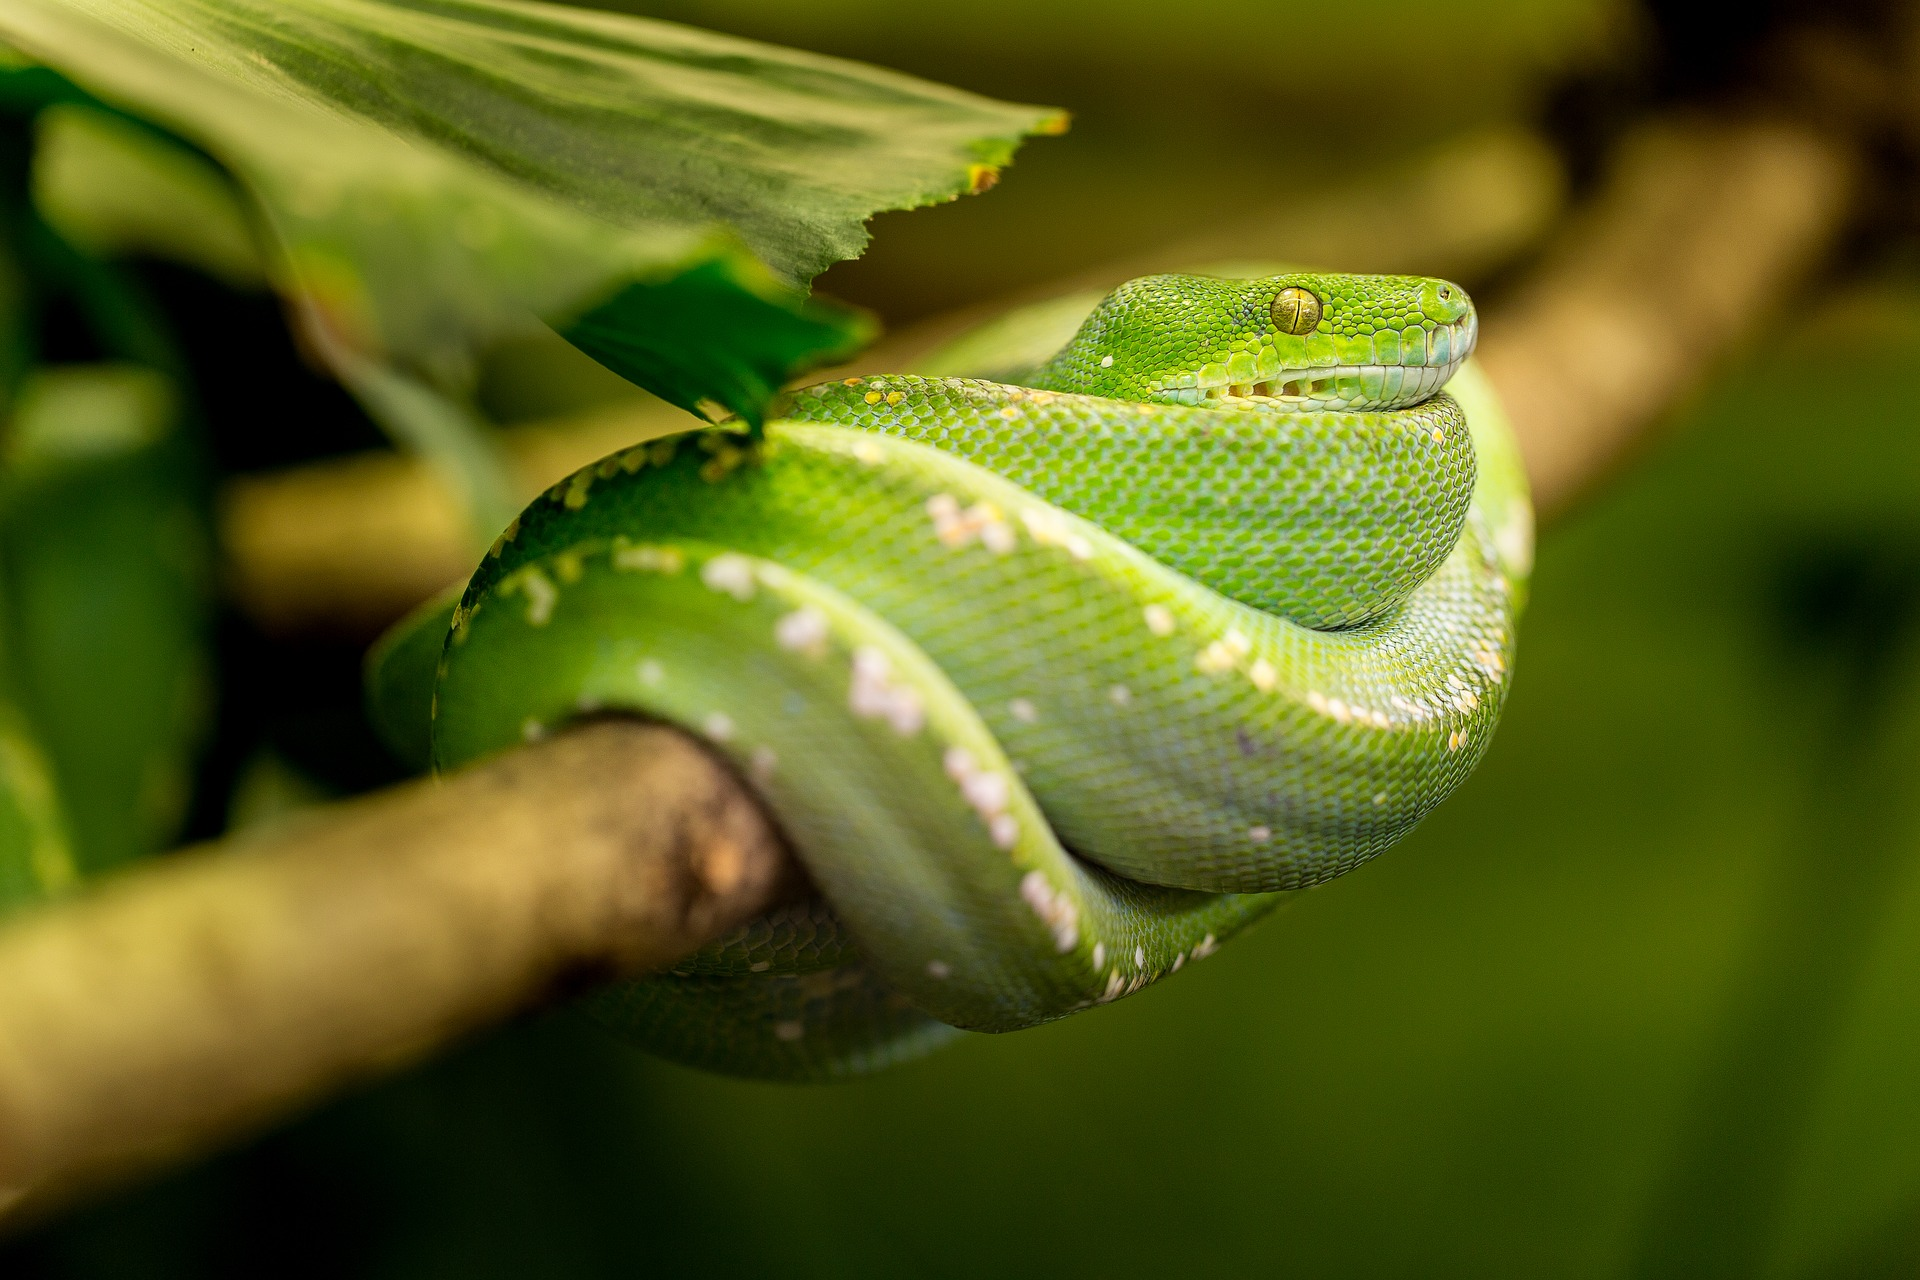
\includegraphics{../images/snake-1634293_1920.jpg}

Getting started in writing programs is easy with Python. It is highly
extensible since there are many add on modules available from a
collection known as Pypi\footnote{\url{https://pypi.org/}} . Python is
fairly easy to learn, epecially when compared to other languges. Python
runs "everywhere", for all intents and purposes. For all these reasons,
Python is a great choice.

An item of note, Python3 is our only choice at this point. Python 2.x
End of Life was January 1st, 2020\footnote{\url{https://github.com/python/devguide/pull/344}}
.

single: Python3

\hypertarget{the-__init__.py-file}{%
\subsection{The \_\_init\_\_.py File}\label{the-__init__.py-file}}

We add this file to let the Python interpreter know that the directories
it is found in are a contiguous part of our Python project. Since module
imports and function definitions in this file are available to all the
python code files in the directory, we can use it to our advantage. For
example, try adding this quick and dirty logging function to
`python/devsecops/lib/\_\_init\_\_.py`:

\begin{Shaded}
\begin{Highlighting}[]
\ImportTok{import}\NormalTok{ logging}
\ImportTok{from}\NormalTok{ pathlib }\ImportTok{import}\NormalTok{ Pathigure logger}

\NormalTok{Path(}\StringTok{"/var/log/devsecops"}\NormalTok{).mkdir(parents}\OperatorTok{=}\VariableTok{True}\NormalTok{, exist_ok}\OperatorTok{=}\VariableTok{True}\NormalTok{)}
\NormalTok{logging.basicConfig(}
\NormalTok{   filename}\OperatorTok{=}\StringTok{"/var/log/devsecops/devsecops.log"}\NormalTok{,}
\NormalTok{   level}\OperatorTok{=}\NormalTok{logging.DEBUG,}
   \BuiltInTok{format}\OperatorTok{=}\StringTok{"[}\SpecialCharTok{%(asctime)s}\StringTok{] [}\SpecialCharTok{%(filename)s}\StringTok{:}\SpecialCharTok{%(lineno)s}\StringTok{ - }\SpecialCharTok{%(funcName)5s}\StringTok{() - }
\StringTok{   }\SpecialCharTok{%(processName)s}\StringTok{] }\SpecialCharTok{%(levelname)s}\StringTok{ - }\SpecialCharTok{%(message)s}\StringTok{"}
\NormalTok{)}
\end{Highlighting}
\end{Shaded}

Now we can create a Python file log\_test.py and call the logger from
within like so:

\begin{Shaded}
\begin{Highlighting}[]
\ImportTok{import}\NormalTok{ logging}
\ImportTok{from}\NormalTok{ pathlib }\ImportTok{import}\NormalTok{ Path}

\KeywordTok{def}\NormalTok{ main():}
\NormalTok{   logging.debug(}\StringTok{'Loggy Loggerton'}\NormalTok{)}
\ControlFlowTok{if} \VariableTok{__name__} \OperatorTok{==} \StringTok{"__main__"}\NormalTok{:}
\NormalTok{   main()}
\end{Highlighting}
\end{Shaded}

Check the results in the file /var/log/devsecops/devsecops.log.

\hypertarget{requirements-file}{%
\subsection{Requirements File}\label{requirements-file}}

A requirements file under python/requirements.txt lists the required
Python modules needed to build and run any Python portions of our
cloudlab project. We also add a check in the Makefile to verify the
existence of the requirements.txt file. The intention is, so we can
quickly cut and paste the Makefile into a new project, but not break
anything if no requirements are present yet.

single: requirements.txt

\hypertarget{test-requirements}{%
\subsection{Test requirements}\label{test-requirements}}

Some requirements are strictly intended to be part of the test harness,
but are not needed for the application proper. Using a separate file,
such as python/requirements-test.txt, makes this delineation clear to
folks who are not familiar with the project.

single: requirements-test.txt

Note that we can also include test requirements in our tox.ini file, as
detailed in the next section.

\hypertarget{project-testing}{%
\subsection{Project Testing}\label{project-testing}}

Security and reliability in our lab and rapid prototyping work is just
as important as it is in our work for the Production environment. In
fact, you might say it's even more important since todays rapid mock ups
can easily wind up making it into the build pipeine when folks are under
a time crunch to deliver.

There are many test frameworks out there, lots of great ideas put forth
by the community. For our current efforts, we've settled on Tox as the
framework of choice. It dovetails nicely with the rest of our patterns.
Tox allows us to manage requirements for virtual environments when
testing, acts as a front end to pytest and coverage modules, and much
more. It is highly configurable and extensible. For example we can test
that an application is compatible with multiple versions of Python.

single: Tox

Use the make test command inside the docker container to run the test
suite for the project.

single: make test

An example tox.ini file follow. Take notice of the "deps" section, where
Python module requirements can be specified. In our current
configuration, these are in lieu of test harness requirements specified
in our python/requirements-test.txt file.

single: tox.ini

\begin{Shaded}
\begin{Highlighting}[]
\NormalTok{[tox]}
\NormalTok{envlist }\OperatorTok{=}\NormalTok{ py38}
\NormalTok{skip_missing_interpreters }\OperatorTok{=}\NormalTok{ true}

\NormalTok{[testenv]}
\NormalTok{setenv }\OperatorTok{=} 
\NormalTok{  PYTHONPATH }\OperatorTok{=}\NormalTok{ .}
\NormalTok{  PYTHONHTTPSVERIFY}\OperatorTok{=}\DecValTok{0} 
\NormalTok{deps }\OperatorTok{=} 
\NormalTok{  coverage}
\NormalTok{  pytest}
\NormalTok{commands }\OperatorTok{=} 
\NormalTok{  coverage run }\OperatorTok{-}\NormalTok{m pytest }\OperatorTok{-}\NormalTok{v }\OperatorTok{--}\NormalTok{capture}\OperatorTok{=}\NormalTok{sys}
\NormalTok{  coverage report }\OperatorTok{--}\NormalTok{omit}\OperatorTok{=}\StringTok{"*/test*,.tox/*"}
\end{Highlighting}
\end{Shaded}

\hypertarget{test-cases}{%
\subsection{Test Cases}\label{test-cases}}

Unit and functional testing is foundational in developing robust, secure
code. We want to be sure that when we create new code, we are also
adding test cases to our test suite that fully cover the new classes,
functions, and so on.

single: Test Cases (Python)

Consider the following example unit test case. The purpose is to test
that the function check\_docker() in the file
python/cloudlab/lib/helper\_functions.py returns True when called from
inside a Docker container.

\begin{Shaded}
\begin{Highlighting}[]
\ImportTok{import}\NormalTok{ pytest}
\ImportTok{from}\NormalTok{ cloudlab.lib.helper_functions }\ImportTok{import}\NormalTok{ check_docker}


\KeywordTok{def}\NormalTok{ test_check_docker():}
   \ControlFlowTok{assert}\NormalTok{(check_docker())}
\end{Highlighting}
\end{Shaded}

\hypertarget{test-coverage}{%
\subsection{Test Coverage}\label{test-coverage}}

As mentioned previously, we can avail ourselves of the coverage module
by adding it to test-requirements.txt or the deps section of our tox.ini
file. The purpose is to automatically generate a report on how much of
our code is "covered" by test cases in python/test.

single: Coverage single: Test Coverage

\hypertarget{python-directory-structure}{%
\subsection{Python Directory
Structure}\label{python-directory-structure}}

Files and folders relevant to the Python portions of our project are
shown in the diagram below.

\begin{description}
\item[digraph folders \{]
1 {[}label="python", shape=folder{]}; 2 {[}label="devsecops",
shape=folder{]}; 3 {[}label="lib", shape=folder{]}; 4
{[}label="requirements.txt", shape=rectangle{]}; 5
{[}label="requirements-test.txt", shape=rectangle{]}; 6
{[}label="\_\_init\_\_.py", shape=rectangle{]}; 7
{[}label="\_\_init\_\_.py", shape=rectangle{]}; 8 {[}label="test",
shape=folder{]}; 9 {[}label="devsecops.py", shape=rectangle{]}; A
{[}label="\_\_init\_\_.py", shape=rectangle{]}; B
{[}label="\_\_init\_\_.py", shape=rectangle{]}; C {[}label="tox.ini",
shape=rectangle{]}; D {[}label="helper\_functions.py",
shape=rectangle{]};

1 -\textgreater{} 2; 1 -\textgreater{} 6; 2 -\textgreater{} 3; 1
-\textgreater{} 4; 1 -\textgreater{} 5; 2 -\textgreater{} 7; 1
-\textgreater{} 8; 2 -\textgreater{} 9; 8 -\textgreater{} A; 3
-\textgreater{} B; 1 -\textgreater{} C; 3 -\textgreater{} D;
\end{description}

\}
